The prototype functionalities focus on the 'line-up' feature, the customer could only retrieve a ticket to enter the store as soon as there is space. The 'book a visit' feature is not implemented.
The scope of the prototype is showing how the system works from the point of view of the customer. For this reason the prototype focuses on the User Experience. The management side is kept at a bare minimum providing only the store operator functions to call customer to the entrance, scan tickets and view real time data about the store crowdedness. The system does not provide functions to insert new stores, neither to create new operator account, but some random data is provided to the testers in order to be able to test the system.
\subsection{Component and Deployment View}
With respect to the Design Document, to ease and speedup the task of developing a prototype some components were moved or removed.
\begin{figure}[h!t]
    \centering
    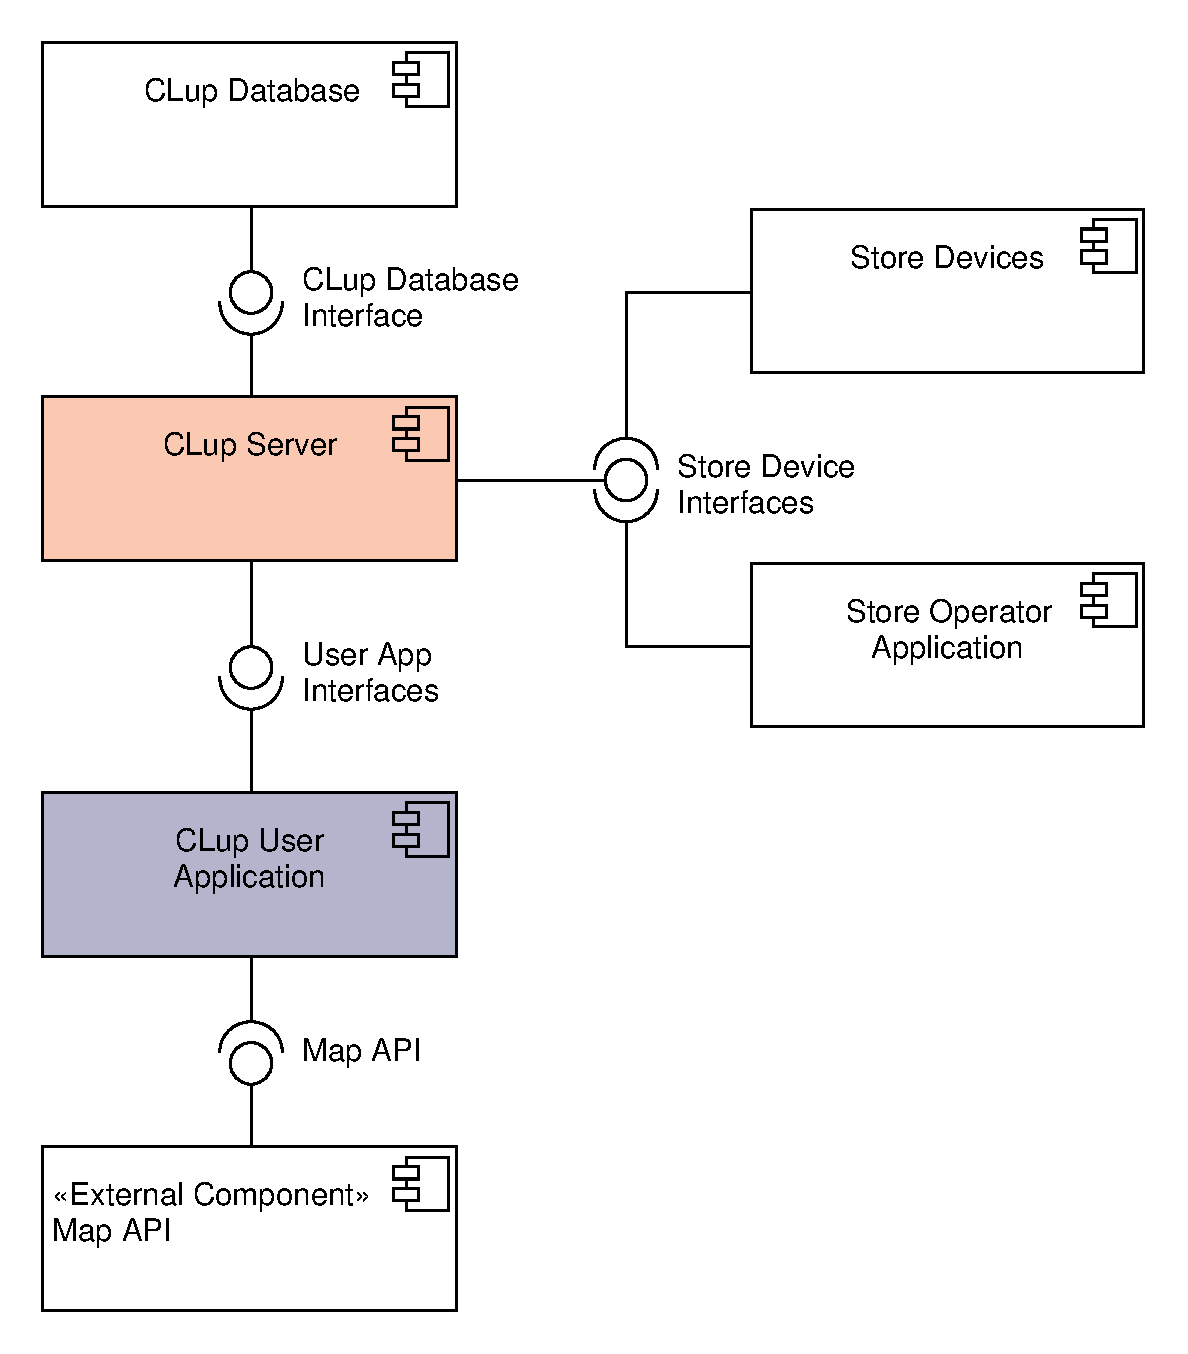
\includegraphics[width=\textwidth]{Images/UML_general_component.pdf}
    \caption{\label{fig:General Component}Implemented Component Diagram}
\end{figure}

\pagebreak

In the DD the original component diagram moved the functions handled from the store out to the CLup server. This is convenient when the two systems handle different types of tickets and different type of statistics to collect but in the case of the prototype there is only one type of ticket to handle. In the prototype is useless to split the two macro components so they are merged in a unique backend macro-component called CLup Server in the diagrams. 
\begin{figure}[h!t]
    \centering
    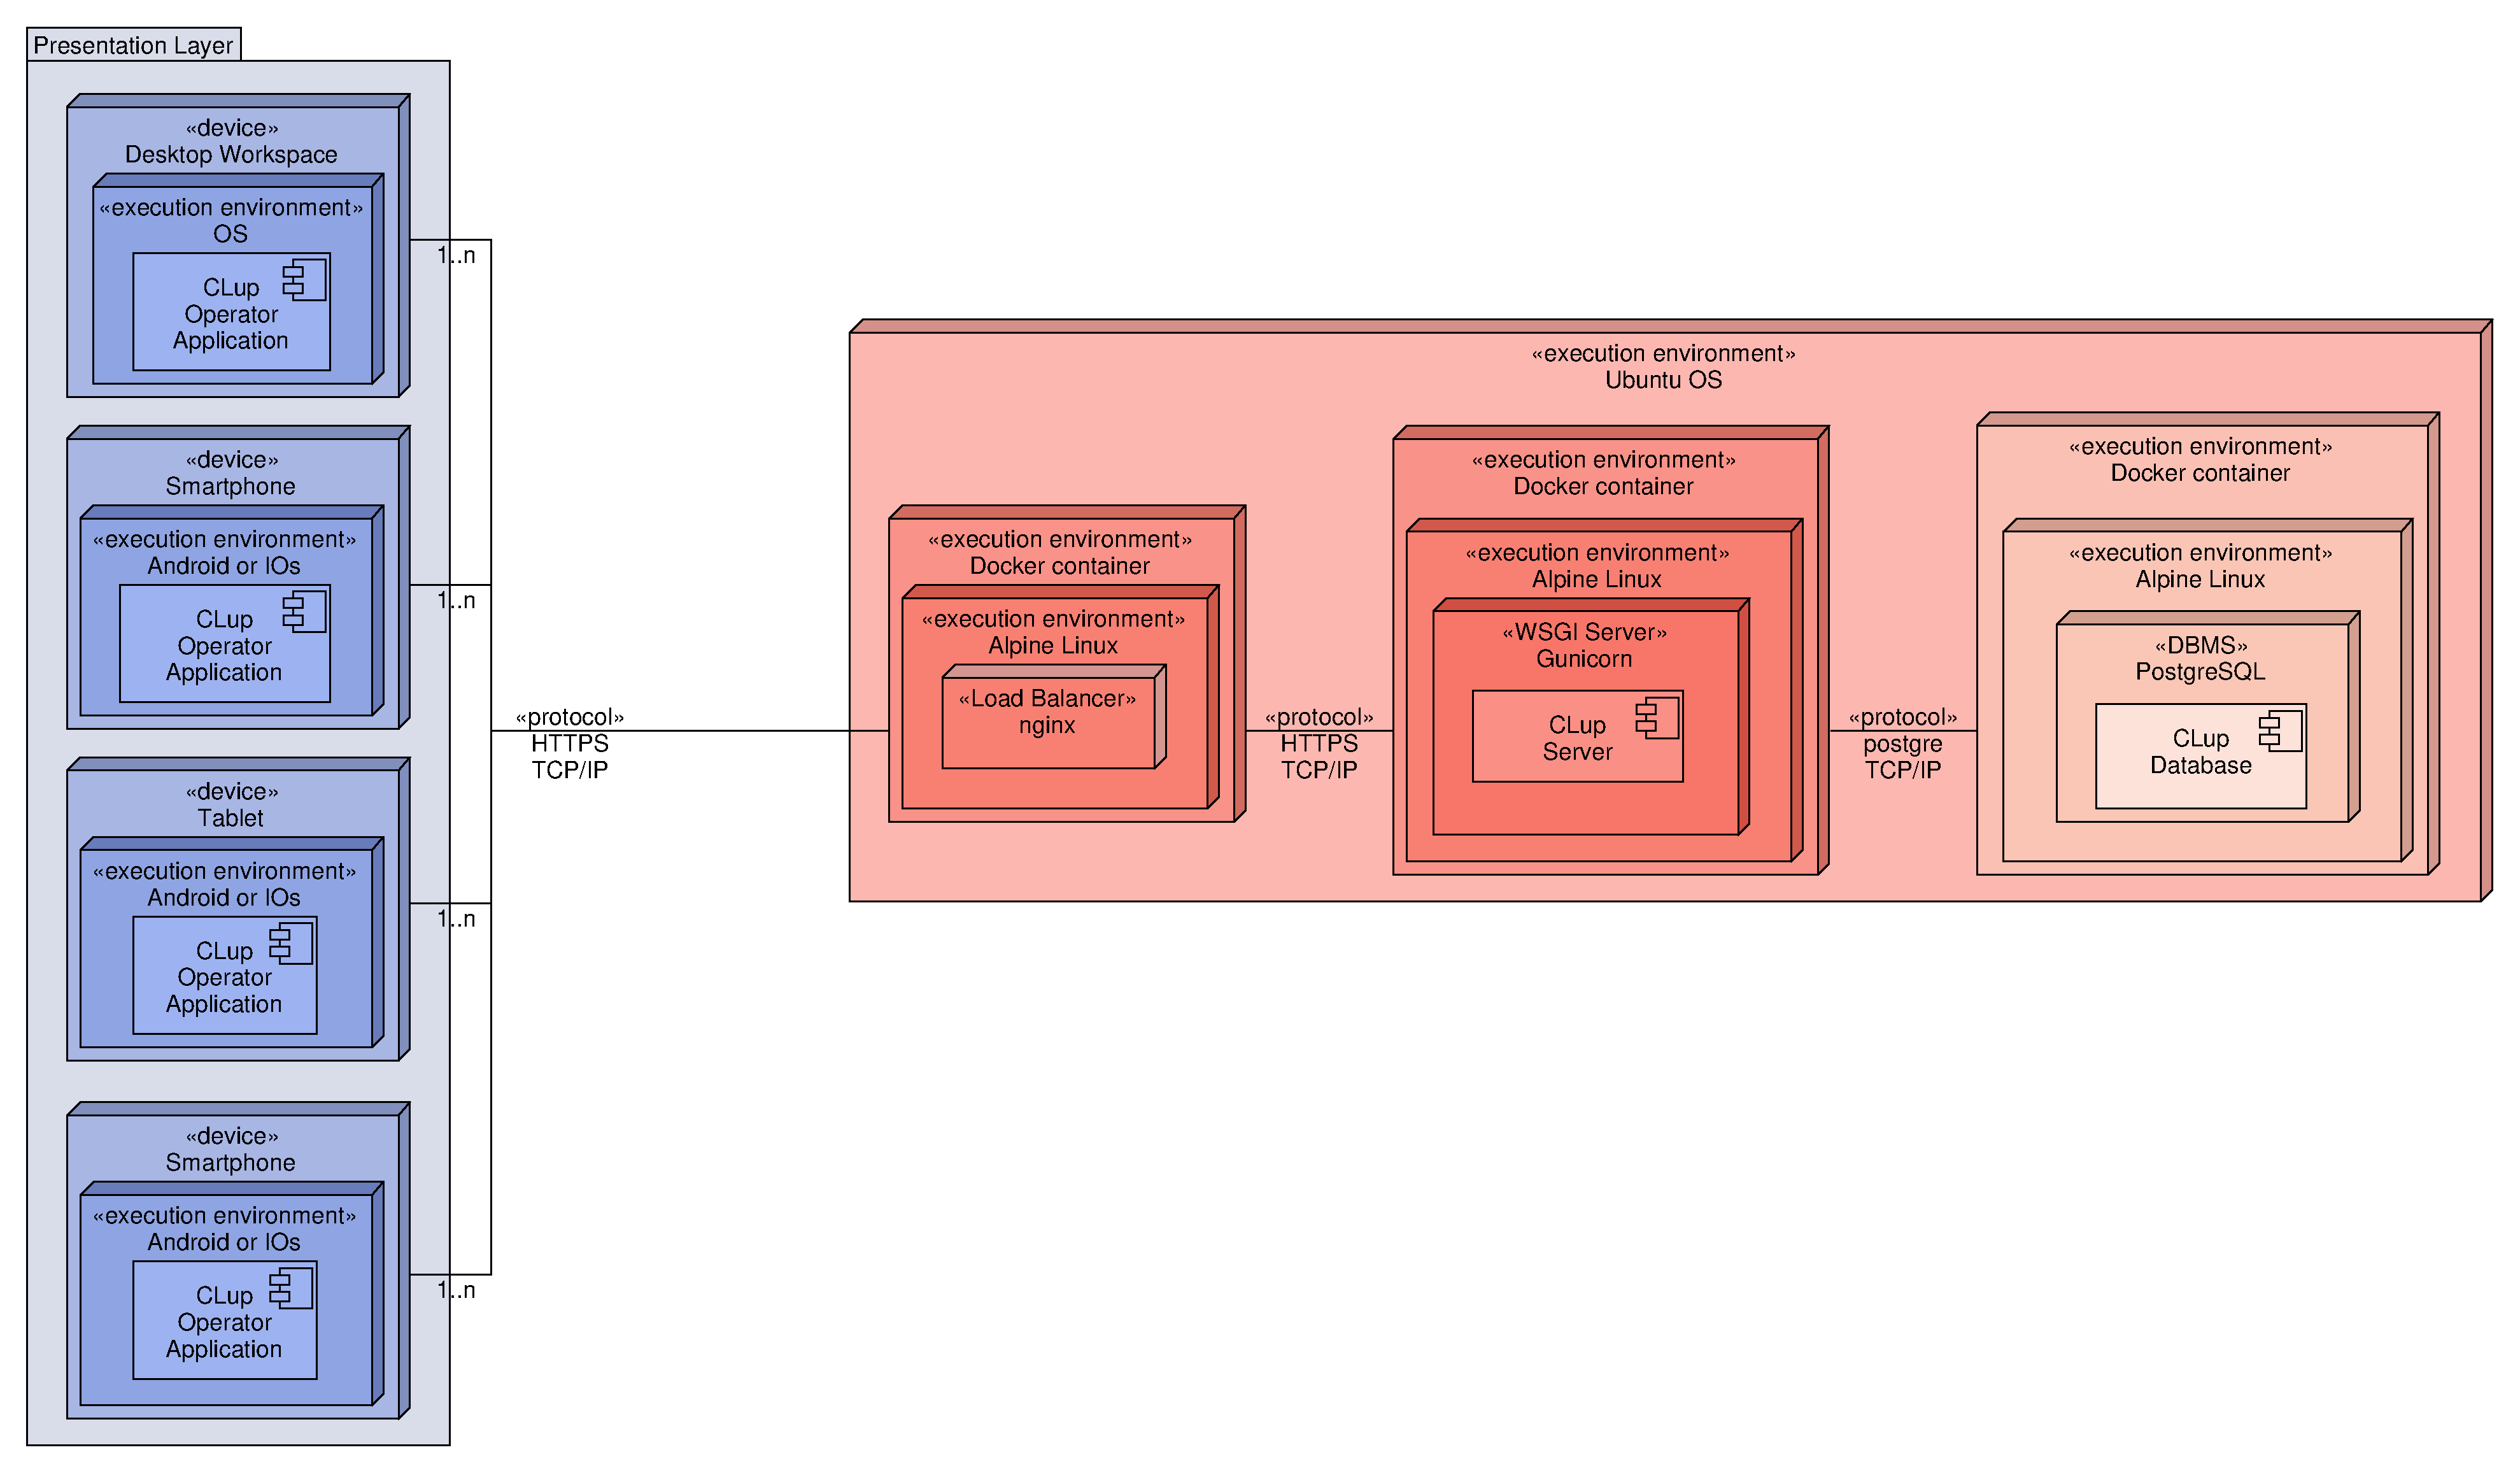
\includegraphics[width=\textwidth]{Images/UML_deployment_diagram.pdf}
    \caption{\label{fig:General Component}Prototype Deployment Diagram}
\end{figure}

Due to the merger of the two components the backend now could run in a single machine isolating the different modules in containers. 



\rowcolors{2}{gray!25}{white}
\renewcommand{\arraystretch}{1.4}
\captionof{table}{Requirements table}
\begin{tabular}{C{1cm}L{11cm}C{3.1cm}}
    \rowcolor{gray!50}
    Label & Requirement description & Implemented?                                                                                                                                                                     \\

    R1   & The system must keep general information and contacts about the store chains adopting CLup & No                                                                                                 \\
    R2   & The system must provide each store a store-admin account  & No                                                                                                                              \\
    R3   & The store-admin account must allow the creation of store-operator accounts &               No                                                                                                   \\
    R4   & For each store the system must allow the users to retrieve information about location and business hours   & Partially                                                                                \\
    R5   & The system stores information about capacity of each market & Yes                                                                                                                                \\
    R6   & The system won't let anyone enter the store if the maximum capacity has been reached  & Yes                                                                                                      \\
    R7   & The system will let a customer enter the store if and only if they have a a valid ticket  & Yes                                                                                                     \\
    R8   & The system will use the occupancy data retrieved from the store to control the store access      & Yes                                                                                    \\
    R9   & The system must provide an interface to communicate with the store access control     & Yes                                                                                                   \\
    R10   & The system must provide an interface for user to compile a shopping list  & No                                                                                                                  \\
    R11   & The system must take in consideration shopping list data and historic data from previous user visits to reduce store crowdedness per department & No                                            \\
    R12   & The system must allow the store-admin account to create and edit entrance time intervals & No                                                                                                   \\
    R13   & Each time interval must have a number of bookable slots fewer than the store capacity & No                                                                                                      \\
    R14   & The system must allow authenticated users to book a visit in a desired time interval & No                                                                                                        \\
    R15   & The system must not allow a user to book a slot in an already full time interval     & No                                                                                                       \\
    R16   & The system must not allow a user to book a visit if he has already reserved another visit  & Yes                                                                                                 \\
    R17   & The system must allow a customer to create a numbered virtual queue ticket and notify them if he can enter immediately (if the store is not full) or provide them a waiting time estimation & Partially\\
    R18   & The system must notify the customers with a virtual queue ticket when it's time to approach the store entrance  & Partially                                                                            \\
    R19   & The store operator application must allow an authenticated operator to manually admit customers & No                                                                                            \\
\end{tabular}

\vfill

\begin{tabular}{C{1cm}L{11cm}C{3.1cm}}
    \rowcolor{gray!50}
    Label & Requirement description & Implemented?                                                                                                                                                          \\
    R20   & The system  must ask the customer to provide the estimated visit time when booking a time slot   & No                                                                               \\
    R21   & The system must allow stores to hand out numbered physical queueing tickets to those that do not use the CLup application & Partially                                                       \\
    R22   & The system must allow the access to the store to customer with numbered tickets using a 'First Come First Served' logic, treating virtual and physical ticket owner equally  & Yes   \\
    R23   & The system must try to estimate waiting time based on store capacity, reservations and the current number of people with numbered tickets waiting in line  & No                      \\
    R24   & The system should interface with an screen placed at the entrance of the store to notify customer which ticket numbers will enter in the next called batch  & Partially                    \\
    R25   & The system must let the store-admin accounts retrieve statistics collected from CLup regarding their store & No                                                                      \\
    R26   & The system must record periodically and store statistics about the occupancy of each store & Yes                                                                                     \\
    R27   & The customer CLup application must show brief statistics about average occupancy of each stores during different days of the week  & No                                             \\
    R28   & The operator CLup application must show to an authenticated operator the real time occupancy of the store & Yes                                                                      \\
    R29   & The customer CLup application must be cross-platform and must work on the majority of the devices & Yes                                                                               \\
    R30   & The stores adopting CLup must be displayed on a map & Yes                                                                                                                            \\
    R31   & The CLup customer application allows user to mark stores as favorite in order to access them quickly                                                                            \\
    R32   & The CLup customer app after the login allows immediately to book tickets right from the homepage & Yes                                                                               \\
    R33   & The system must provide an interface for automated control devices to communicate to CLup data about store entrances, store leavings and crowdedness in the various departments & Partially\\
    R34   & The system must push notifications to user devices with update information on the store he has a ticket for   & Partially                                                                  \\
    R35  & The system must associates tickets with line numbers & Yes                                                                                                                           \\
    R36  & The system allows customer to register an user account & Yes \\
    R37  & The system allows registered customers to authenticated & Yes\\
\end{tabular}
\vfill
\subsection{Partially Implemented Features}
\begin{itemize}
    \item \textbf{R4 For each store the system must allow the users to retrieve information about location and business hour}: The store location feature is implemented (in order to display stores in the map). The business hours are not provided to the user, this feature could be implemented using an external API with opening times or storing these opening times in the database
    \item \textbf{R17 The system must allow a customer to create a numbered virtual queue ticket and notify them if he can enter immediately (if the store is not full) or provide them awaiting time estimation}: The waiting time estimation is not provided. To estimate the waiting time an accurate model based on historical data could be used.
    \item \textbf{R18 The system must notify the customers with a virtual queue ticket when it’s time to approach the store entrance}:
    The push notification component is not implemented in the prototype so the server can't push message to the user application. However the client will check if the ticket has been called by pulling data from the server API periodically.
    \item \textbf{R21 The system must allow stores to hand out numbered physical queueing tickets to those that do not use the CLup application}:
    The CLup server provides an API for this feature but for satisfying this requirement a ticket printer is required. 
    \item \textbf{R25 The system should interface with an screen placed at the entrance of the store to notify customer which ticket numbers will enter in the next called batch}:
    Similar to R21
    \item \textbf{R33 The system must provide an interface for automated control devices to communicate to CLup data about store entrances, store leavings and crowdedness in the various departments}: Similar to R21. The departments' crowdedness control feature is not implemented in the prototype



\end{itemize}

